\chapter{Visão Geral do Sistema}

\section{Visão Geral Do Subsistema de Software}

O subsistema de \textit{software} é composto por um \textit{webapp} e o \textit{webservice} com o qual o web app faz e o \textit{raspberry} fará a comunicação. Na seção do webapp para o cliente é possível fazer a compra do picolé e a liberação do mesmo, por meio de um botão que se comunica com o \textit{webservice}, que por sua vez comunicará com o \textit{raspberry}, dando o comando para liberação do picolé. A seção do \textit{webapp} para o vendedor terá funções de administrador, podendo aumentar o estoque quando recarregar a máquina de vendas, além de o administrador poder cadastrar vendedor e máquina.

\begin{figure}[H]
	\centering
    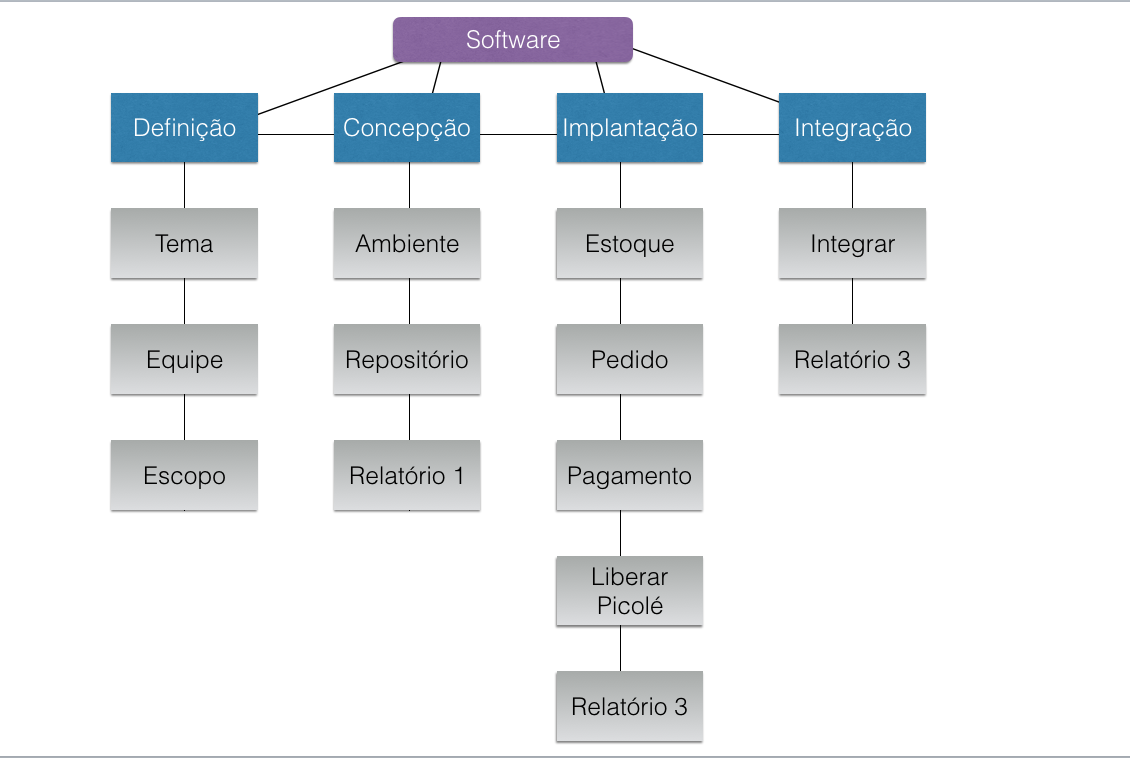
\includegraphics[width=\textwidth]{figuras/vg_software}
    \caption{Diagrama de Software}
    \label{fig:vg_software}
\end{figure}

\newpage

\section{Visão Geral Do Subsistema de Eletrônica}

A visão geral do subsistema eletrônico, consiste no controle geral feito pela Raspberry PI 3 e na sua comunicação com o Arduino UNO. Na integração entre software e hardware via GPRS e na aquisição de dados da localização (GPS), informação a qual é utilizada no sistema de segurança de furto e extravio. O sistema de sensoriamento e controle de recepcionamento do cliente (som e interface) também é submetido por tais controladores, devido à sua alta capacidade de processamento e facilidade de comunicação. O diagrama da atividade eletrônica é mostrado na figura \ref{fig:diagrama} a seguir:

\begin{figure}[H]
	\centering

    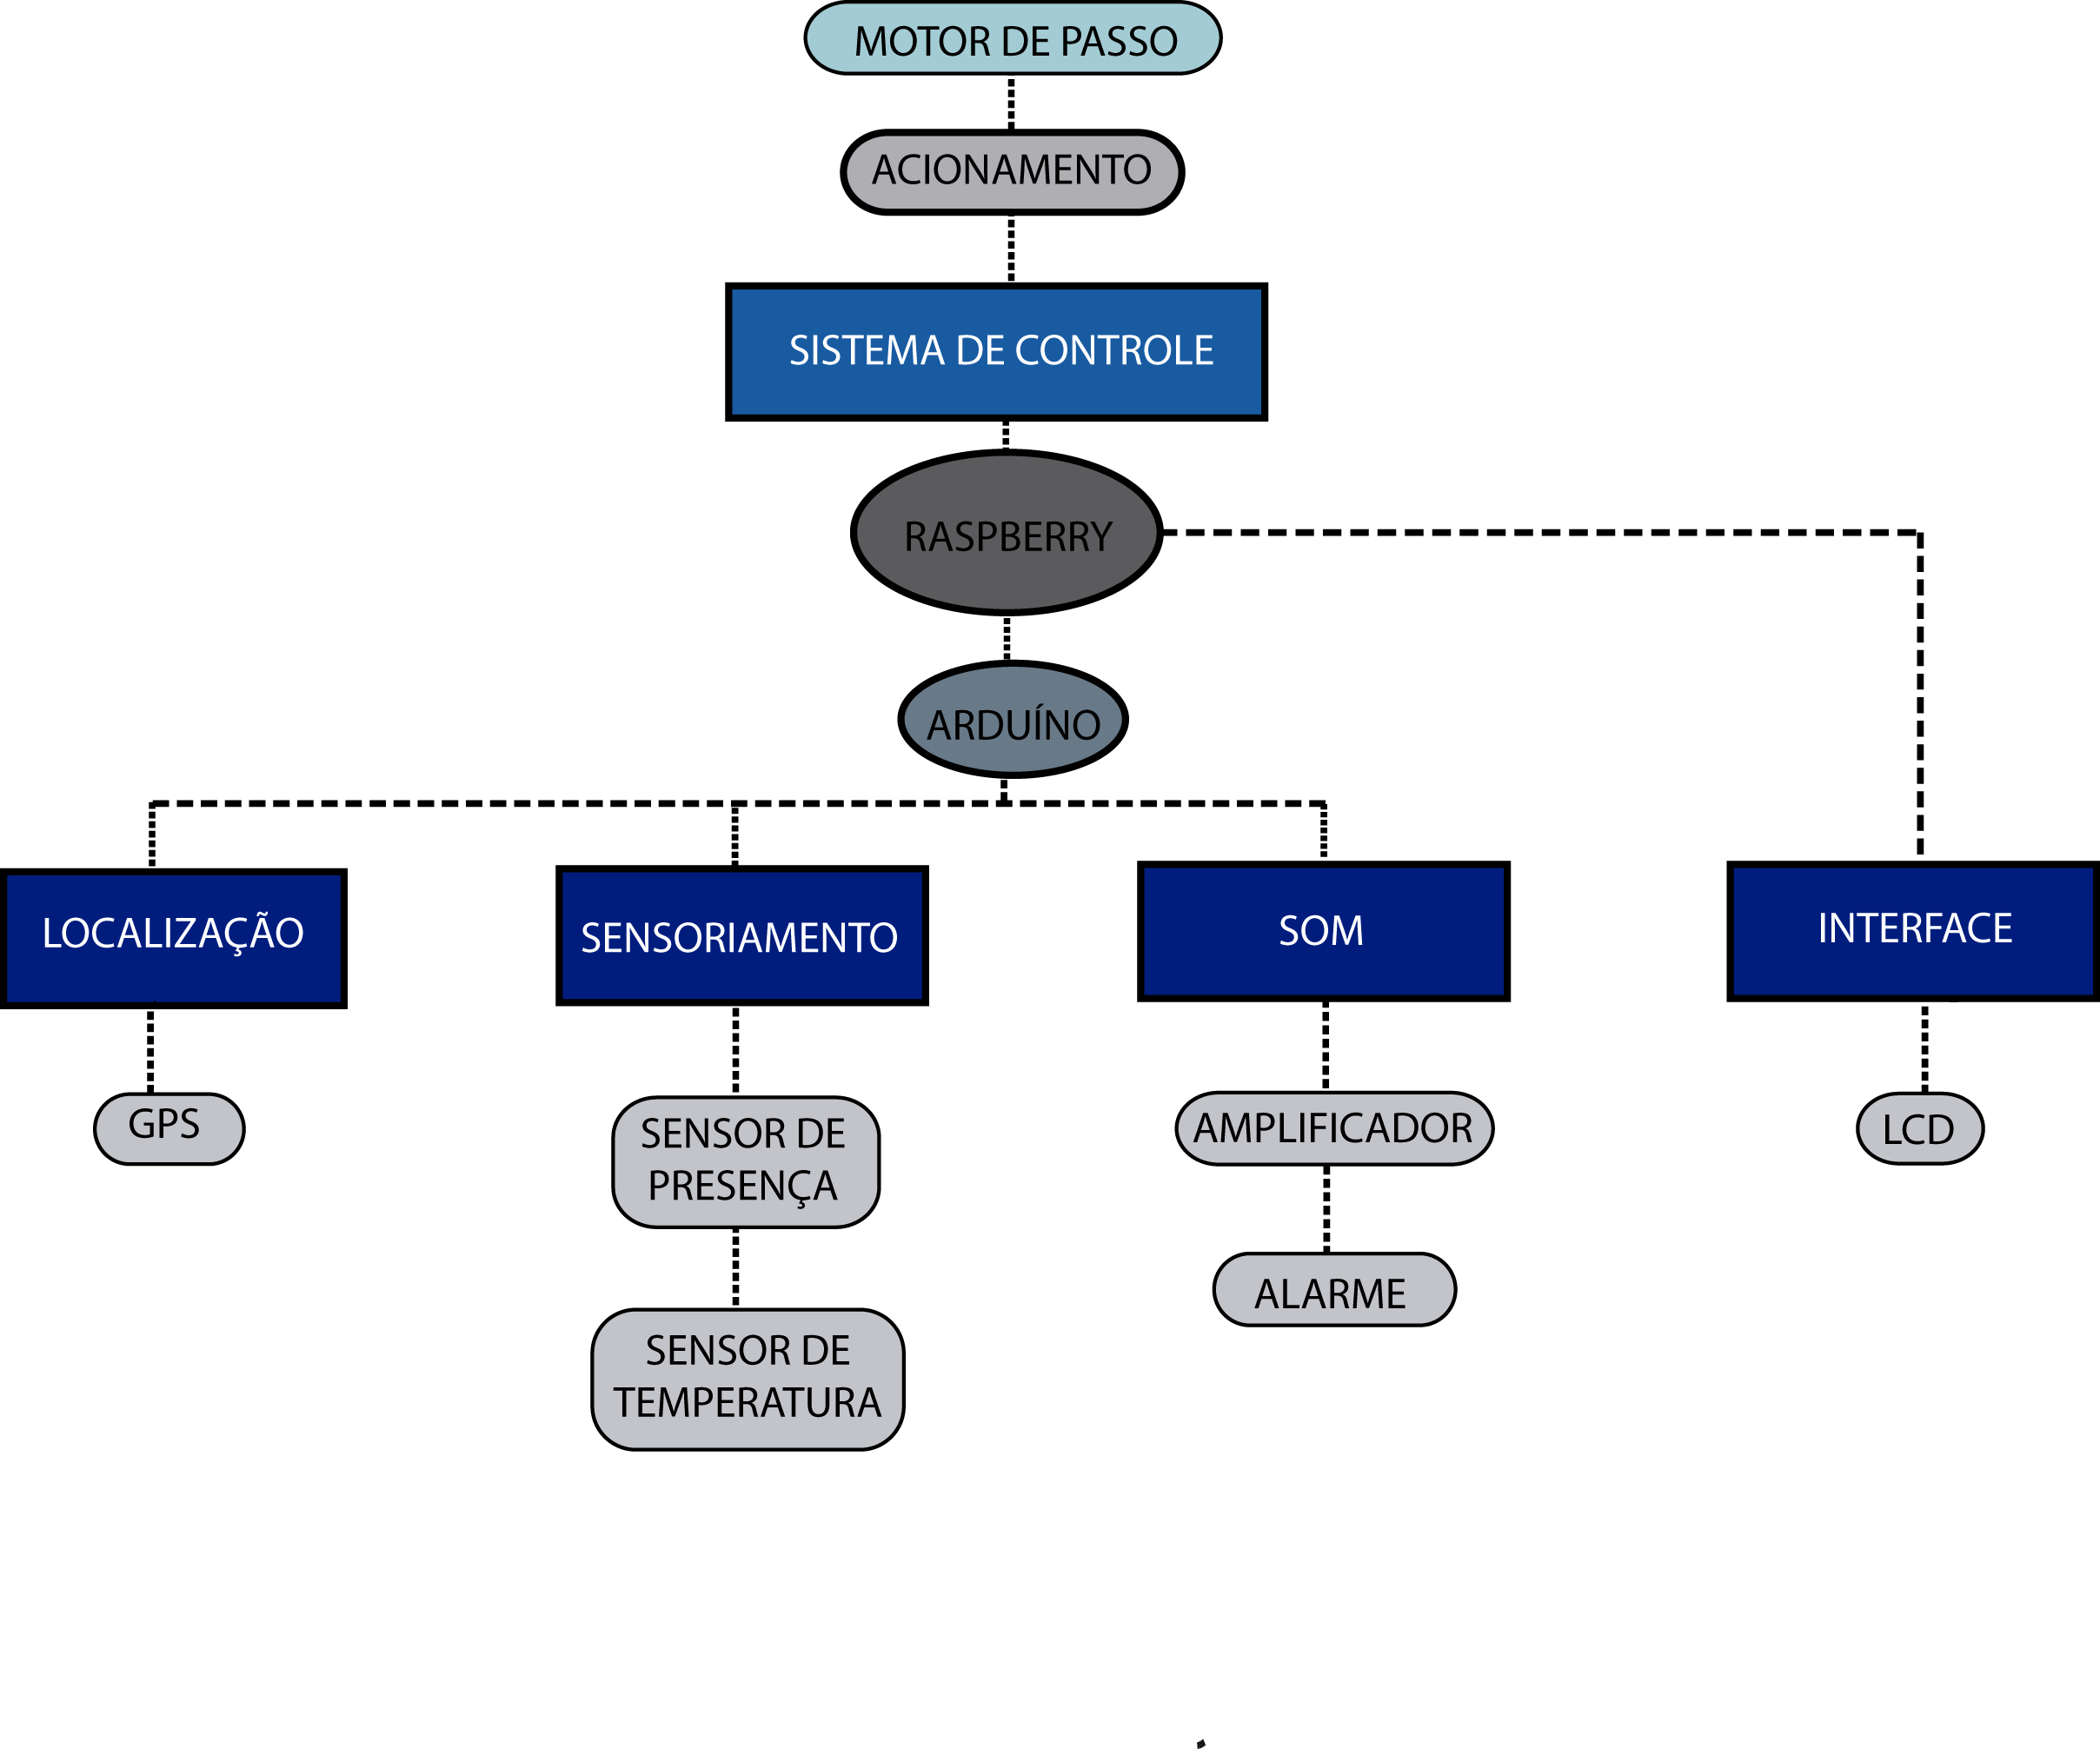
\includegraphics[width=1.05\textwidth]{figuras/diagrama}
    \caption{Diagrama da estrutura eletrônica do produto}
    \label{fig:diagrama}
\end{figure}

\newpage

\section{Visão Geral Do Subsistema de Estruturas}

A visão geral das estruturas do projeto é dividida pelos componentes que necessitam ser construídos, fixados e integrados. São eles: mecanismos para entrega do picolé, estrutura de suporte das placas solares, carrinho de transporte da máquina de venda e os compartimentos internos da máquina de venda (\textit{freezer}, componentes eletrônicos, bateria e compressor).

\begin{figure}[H]
	\centering

    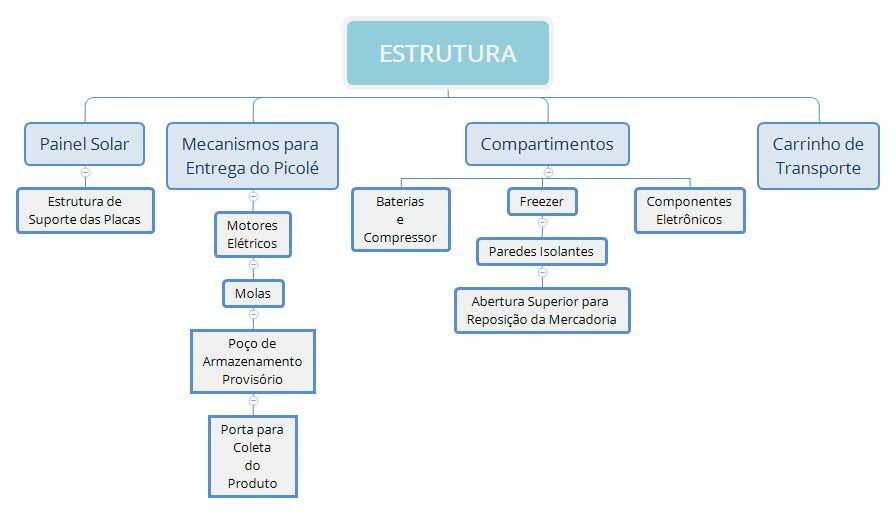
\includegraphics[width=\textwidth]{figuras/Vis_o_Geral_-_ESTRUTURA}
    \caption{Diagrama das estruturas}
    \label{fig:Vis_o_Geral_-_ESTRUTURA}
\end{figure}

\newpage

\section{Visão Geral Do Subsistema de Energia}

	A visão geral do subsistema de energia, consiste no fornecimento de informações voltado para a alimentação dos sistemas consumidores de energia primária (refrigerador) e periféricos (iluminação, carregador de tablet, motores, sistema eletrônico, entre outros), bem como, o dimensionamento do painel fotovoltaico,  \textit{pack} de baterias, inversor e controlador de carga.

  \begin{figure}[H]
	\centering

    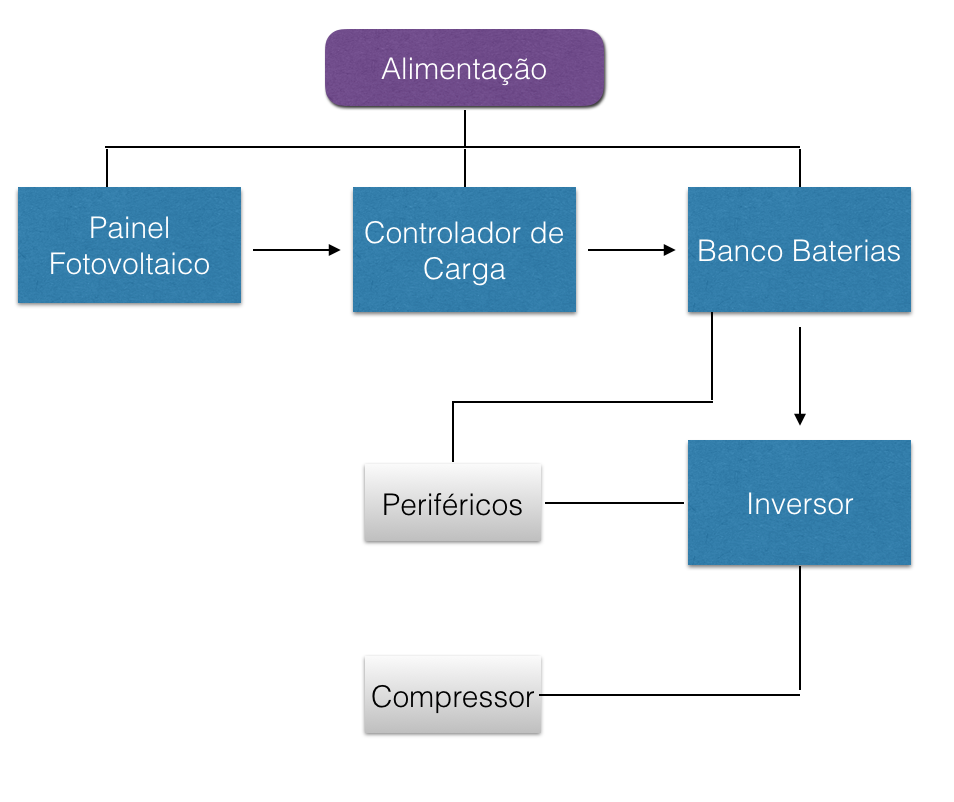
\includegraphics[scale=0.8]{figuras/diagrama_energia}
    \label{fig:diagrama_energia}
    \caption{Diagrama energia}
\end{figure}

	O sistema foi dimensionado com um fator de segurança elevado, para que a \textit{Vending Machine} entregasse a confiabilidade de um produto passível de comercialização. Para isso, a bateria teve em seu dimensionamento a consideração do tempo de operação do serviço relacionado diretamente com o consumo da bateria. O inversor utilizado para o projeto foi dimensionado considerando as cargas exigidas, principalmente pelo compressor, o qual é o principal consumidor do produto.
